\documentclass[12pt]{beamer}

\usepackage{beamerthemeHannover, graphicx, clrscode, amsmath, amssymb, multicol}
\setbeamercolor{sidebar}{use=structure,bg=gray!20!green!60!white}

\title{Scientific Computing With Perl and Math::GSL}
\author[J.A. Leto]{Jonathan Leto\\jonathan@leto.net}
\date{}

\begin{document}
\frame{
    \titlepage
    \begin{center}
    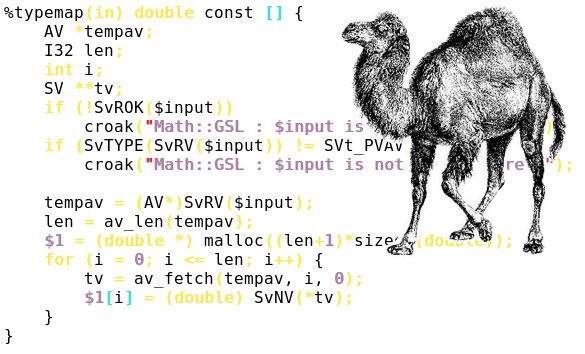
\includegraphics[width=5.84cm, height=3.85cm]{swig_camel}
    \end{center}
}

\section{Why do "Science" with Perl?}
\frame{
    \frametitle{Why do "Science" with Perl?}
    \begin{center}
    \begin{itemize}
        \item CPAN - Don't reinvent the wheel
        \item Data Munging - 
        \item Camels are cool
    \end{itemize}
    \end{center}

}

\section{Basic Tools}
\frame{
    \frametitle{Basic Tools}
    \begin{center}
    \begin{itemize}
        \item PDL - Perl Data Language
        \item Math::GSL - Interface to the GNU Scientific Library
    \end{itemize}
    \end{center}
}

\section{Going Forward}

\frame{
    \frametitle{Active Development Continues}

    \begin{itemize}
        \item Scientific Computing applications built on top of Math::GSL
        \item Math::Symbolic integration
        \item PDL integration
        \item Callbacks and threaded Perls
    \end{itemize}
}
\section{Acknowledgements}
\frame{
    \frametitle{Thanks}

    \begin{itemize}
        \item Eric Wilhelm
        \item Thierry Moisan
        \item \#pdx.pm
    \end{itemize}
}

\frame{
    \frametitle{More Info}
    \begin{itemize}
        \item {http://leto.net/gitweb/}\\
        \item {http://leto.net/code/Math-GSL/}\\
        \item {http://groups.google.com/group/math-gsl-dev}\\
        \item {http://groups.google.com/group/perl-scientific-computing}\\
    \end{itemize}

}

\end{document}
